\chapter{Linux相关笔记}

\section{linux备忘录}

以下零零散散的一些笔记用于记录不太熟的Linux指令,不断扩充中……
\begin{enumerate}
  \item 永久修改ip地址。首先ifconfig找到对应的网卡,其次编辑 vi /etc/sysconfig/network-scripts/ifcfg-lo,此处假设网卡是lo。
  \item 当我们输入history的时候,会出现历史命令。这些命令从1开始到history这个指令的索引数,可以用!+index的方式来调用。比如history中显示的第五条命令是ls,那么当我们在终端输入 !5 的时候会自动调用 ls 指令。而且 ! 也可以接指令的部分内容,其会自动找寻最近的一条与该内容相关的指令并执行。比如说历史中有两条 ls 指令。一条是ls / ;一条是ls /home,假设第二条是最近的指令,那么我们执行 !ls,那么系统就会执行 ls /home 这条指令。
  \item alias short\_cmd='real\_cmd',使用这个指令可以将real\_cmd用short\_cmd代替,减少常用命令的输出时间。使用unalias short\_cmd可以取消对应的映射。alias单独运行可以查看当前有哪些short\_cmd。而且我们可以将这个指令直接添加到 \~/.bashrc中,这样就万事大吉,省心了,重启的时候也不会消失。
  \item > >> 2> 和 2>> 还有 &>  bash run.sh 1>>result 2>&1。 正确错误的都会传到result里面。
  \item free -m 以M为单位显示磁盘存储空间
  \item 修改Ubuntu下载源可以修改 /etc/apt/sources.list 文件
  \item 查看Ubuntu版本可以使用 cat /etc/issue
  \item Ubuntu下解决ifconfig command not found的办法:sudo apt-get install net-tools
  \item 当拥有多个用户,想把某个文件或者文件夹的权限下放到某个用户或者限制某个用户对某个文件或者文件夹的访问的时候,可以使用 setfacl 这个指令。具体的下放权限指令操作为: setfacl -m u:user1:rw test.txt,清空对于某个文件或者文件夹设置的权限时指令操作为: setfacl -b  test.txt。查看某个文件或者文件夹更细化的权限信息可以使用 getfacl 指令。对目录以及子目录设置acl权限时,指令为:setfacl -m u:user1:rw -R /mnt。如果后续当前目录有生成新的子目录或者文件,想要继承现有权限的时候,需要在执行上述指令之后,再执行一次 setfacl -m d:u:user1:rw -R /mnt
  \item 设置用户对于某个命令的执行权限,使用指令 visudo(需要在root下执行),举例:首先执行visudo,会打开一个文件,要添加某个用户对于某个指令的权限时,需要给出对应命令的绝对路径,假设给予 user4 添加新用户的权限,则在visudo打开的文件添加一句 user4 localhost=/usr/sbin/useradd,之后使用 sudo /usr/sbin/useradd user5 之后再输入 user4 的密码,就可以创建 user5。多个命令使用 “,” 隔开。
  \item 分配无密码的sudo命令:同样使用 visudo,然后在文本中添加一句: user4 ALL=NOPASSWD: /usr/sbin/useradd, /usr/sbin/userdel,之后再调用 sudo /usr/sbin/useradd user5 的时候就不需要 user4 的密码了。也可以使用 user4 localhost=NOPASSWD: /usr/sbin/useradd, /usr/sbin/userdel,这就意味着只有在 user4 下的时候才可以不用输入密码,而 ALL 表示在所有用户下使用 sudo 都不用输入密码。
  \item 任务计划  crontab -e 创建一个新的任务计划。 30 17 * * 5 task,其中前面的表示周五的17:30,在这个时间点执行任务task。可以用 crontab -l 查看任务计划的内容。
  \item ls -R 递归式的显示当前目录所有的东西,包括文件,子目录,子目录中的所有东西
  \item 创建一个ftp服务站代码如下,这个时候在/var目录下会生成一个ftp的目录,ftp下还有个pub目录,这个目录,使得我们可以在其他操作系统访问。在Windows下,打开文件夹,在文件栏输入ftp://your\_ip即可访问ftp的pub目录,ftp启动指令为 service vsftpd start。
  \begin{lstlisting}[language = shell, numbers=left, 
         numberstyle=\tiny,keywordstyle=\color{blue!70},
         commentstyle=\color{red!50!green!50!blue!50},frame=shadowbox,
         rulesepcolor=\color{red!20!green!20!blue!20},basicstyle=\ttfamily]
yum -y install vsftpd*
  \end{lstlisting}
  \item 查看linux某个端口是否被占用指令:netstat -anp|grep \$port
  \item 当我们不需要显示输出结果,但是Linux指令默认自动输出指令的时候,我们可以在指令后面加上 \&>/dev/null,这样所有输出就重定向到一个黑洞里,全部都消失了。
  \item \textcolor{red}{解决Linux中文乱码问题}:以docker安装的Ubuntu为例。
   \begin{lstlisting}[language = shell, numbers=left, 
         numberstyle=\tiny,keywordstyle=\color{blue!70},
         commentstyle=\color{red!50!green!50!blue!50},frame=shadowbox,
         rulesepcolor=\color{red!20!green!20!blue!20},basicstyle=\ttfamily]
>>locale -a
C
C.UTF-8
POSIX
>>export LC_ALL='C.UTF-8'  #这是临时修改的
>>export LC_ALL='C.UTF-8' >> /etc/bash.bashrc | source /etc/bash.bashrc  #这是永久修改。
>> docker restart <container-ip>  #退出container,重启container即可
  \end{lstlisting} 
  \item docker启动命令: systemctl start docker
  \item \textcolor{red}{bad interpreter: No such file or directory}:出现这个错误的原因是我用winscp连接服务器,然后用Windows系统下的VScode写代码。因为Windows下文本默认的格式是DOS,而Linux是unix,所以在服务器上运行的时候会出现这个错误。修改的办法有两个:第一个是在Linux里面用vim打开这个脚本,输入 set ff 的时候会出现个DOS,所以我们要设置下属性,如下所示。另外我们还可以在VScode中直接修改,写好脚本之后,点击右下角的CRLF,上边栏会出现一个选项,选择LF即可,如图\ref{fig:lf-crlf}。
   \begin{lstlisting}[language = shell, numbers=left, 
         numberstyle=\tiny,keywordstyle=\color{blue!70},
         commentstyle=\color{red!50!green!50!blue!50},frame=shadowbox,
         rulesepcolor=\color{red!20!green!20!blue!20},basicstyle=\ttfamily]
:set ff=unix
  \end{lstlisting}  
\begin{figure}[h]
  \centering
  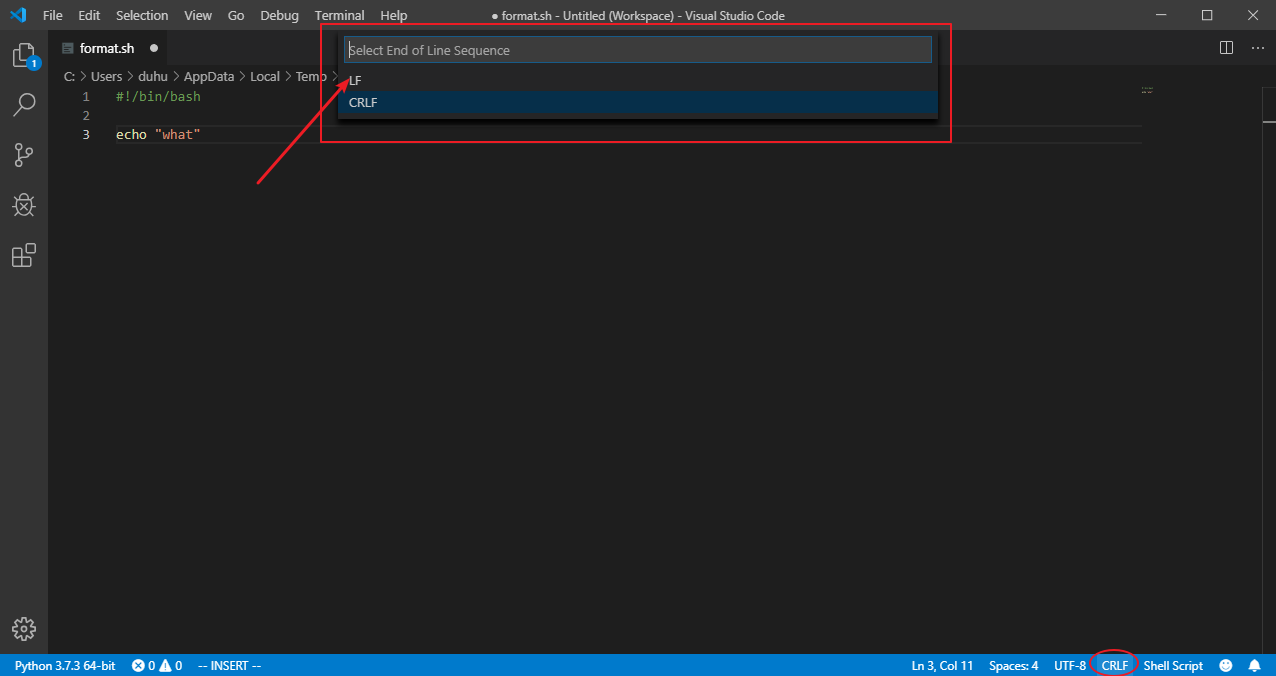
\includegraphics[width=0.7\textwidth]{lf-crlf}
  \caption{VScode设置脚本格式为Unix \label{fig:lf-crlf}}
\end{figure}
  \item 我们在Linux上安装软件时,经常需要选择机器所对应的版本,即机器是多少位的。查看指令有:
    \begin{itemize}
      \item uname -a
      \item file /bin/ls
      \item cat /proc/vision
      \item getconf LONG\_BIT
    \end{itemize}
  \item 删除文本中的空行:grep -v '^$' file
  \item 如何对文本指定列进行排序:
  \begin{lstlisting}[language = shell, numbers=left, 
         numberstyle=\tiny,keywordstyle=\color{blue!70},
         commentstyle=\color{red!50!green!50!blue!50},frame=shadowbox,
         rulesepcolor=\color{red!20!green!20!blue!20},basicstyle=\ttfamily]
sort -n -k2 file  #numerical sort;k2表示的是某一列,从小到大排序
sort -g -k2 file  #general-numerical sort
sort -nr -k2 file #从大到小排序
  \end{lstlisting}  
  \item 出现错误:"[: too many arguments":这个是在字符串比较中出现的,表示的是比较的对象数量不一致,也就是说可能出现多个字符串,这个时候给这个变量添加上双引号就可以了。
\end{enumerate}

\section{Shell指令笔记}

\subsection{简单的shell规则}
此处记载一些简单的shell指令和编程规则。不断补充……
\begin{enumerate}
  \item 将键盘输入的内容赋值给变量: read [-p "some message"] 变量名。
  \item 双引号("")允许通过\$符号引用其他变量值;单引号('')禁止引用其他变量值,\$视为普通字符;反撇号(\`\`)将命令执行的结构输出给变量。
  \item 关于shell中外部传输变量的一些操作:
    \begin{itemize}
      \item \$\#:命令行中位置参数的个数;
      \item \$*:所有位置参数的内容,当格式为"\$*"时,参数作为一个整体传递给程序;
      \item \$?:上一条命令执行后返回的状态,当返回状态值为0时,表示执行正常;非0则表示执行异常;
      \item \$0:当前执行的进程/程序名;
      \item \$n:$n\in\{0,1,2,3,4,5,6,7,8,9\}$,表示外部传入的第n个参数。
      \item \$@:传递所有参数的内容,当格式为"\$@"的时候,表示将参数分开传递给程序;
    \end{itemize}
  \item shell中的数学运算指令:expr。注意乘法是 $\backslash$*
  \item 解析字符串中的转义字符,可以使用 echo -e,比如 echo -e "test$\backslash$ntest",echo -e 还可以修改输出的颜色和背景色,指令是$\backslash$[033[前景颜色;背景颜色m。$\backslash$[033[0m 表示恢复到系统默认颜色。其前景颜色的数值为:默认=0,黑色=30,红色=31,绿色=32,黄色=33,蓝色=34,紫色=35,天蓝色=36,白色=3;背景颜色的数值为:默认=0,黑色=30,红色=31,绿色=32,黄色=33,蓝色=34,紫色=35,天蓝色=36,白色=3。
  \item shell默认在输出之后换行的,如果想要不换行,可以选择参数 -n。例如echo -n "Enter your name: ",这样在终端显示的时候就不会换行。只有一个echo的时候,会输出一个换行。
  \item cat的另外一种用法,比如可以用于制作菜单,如下程序所示,这个程序在执行的时候会保留原样输出两个x之间的内容,包括换行和空格等。
    \begin{lstlisting}[language = shell, numbers=left, 
         numberstyle=\tiny,keywordstyle=\color{blue!70},
         commentstyle=\color{red!50!green!50!blue!50},frame=shadowbox,
         rulesepcolor=\color{red!20!green!20!blue!20},basicstyle=\ttfamily]
cat<<x
  please input your name:
      1) user1
      2) user2
      3) user3
x
    \end{lstlisting}
  \item \textcolor{red}{nl} 指令:给输出标上行,比如 cat test.txt | nl,这条指令会给test.txt中的每一行进行顺序标号;
  \item \textcolor{red}{tee} 指令:在程序执行输出的时候额外保留一份输出到文件中,比如 ./test.sh | tee test.txt。能够起到一个备份的作用。
  \item \textcolor{red}{shift} 指令:用于迁移位置变量,将\$1到\$9依次向左传递。
  \item 两个文件的交集、并集和去重:
    \begin{lstlisting}[language = shell, numbers=left, 
         numberstyle=\tiny,keywordstyle=\color{blue!70},
         commentstyle=\color{red!50!green!50!blue!50},frame=shadowbox,
         rulesepcolor=\color{red!20!green!20!blue!20},basicstyle=\ttfamily]
cat file1 file2 | sort | uniq > result   #求两个文件的并集,如果有重复的行只保留一行。 
cat file1 file2 | sort | uniq -d > result #求两个文件的交集,即两个文件中都有的行。
cat file1 file2 | sort | uniq -u > result #求两个文件的差集,即只有一个文件中有的行。
cat file1 file2 > result #追击的方式,如果file1有n行,file2有m行,result为n+m行
paste file1 file2 > result  #一个文件的内容在左边,一个文件命令在右边。
sort file |uniq #将重复的多行变为一行
sort file |uniq -u #sort file |uniq -u
    \end{lstlisting}
\end{enumerate}

\subsection{shell中的条件测试操作}
\begin{enumerate}
  \item \textcolor{blue}{test命令}:
    \begin{enumerate}
      \item 用途:测试特定的表达式是否成立,成立返回0,不成立则返回非0;
      \item 格式: test 条件表达式 [ 条件表达式 ]
    \end{enumerate}
  \item \textcolor{blue}{常见的测试类型}
    \begin{enumerate}
      \item 测试文件状态:
        \begin{itemize}
            \item 格式: [ 操作符 文件或者目录 ]
            \item 常用的文件操作符,如表\ref{tab:test_sign}。
              \begin{table}[h]
               \centering
               \caption{常用的文件操作符及其意义}
                 \begin{tabular*}{1\textwidth}{@{\extracolsep{\fill}}cc}
                 \toprule
                 文件操作符     &作用                            \\
                 \midrule
                 -d            &是否为目录(Directory)          \\
                 -f            &是否为文件(File)               \\
                 -e            &是否存在文件或者目录(Exist)     \\
                 -r            &当前用户是否可读(Read)          \\
                 -w            &当前用户是否可写(Write)         \\
                 -x            &当前用户是否可操作(Excute)      \\
                 -L            &文件是否为符号链接文件(Link)     \\
                 \bottomrule
                 \end{tabular*}%
               \label{tab:test_sign}%
              \end{table}%
            \end{itemize}
      \item 字符串比较:
        \begin{itemize}
                \item 格式: [ 字符串1 = 字符串2 ], [ 字符串1 != 字符串2 ],[ -z 字符串]
                \item 常用的字符串操作符,如表\ref{tab:test-str}。
                  \begin{table}[h]
                   \centering
                   \caption{常用的字符串操作符及其意义}
                     \begin{tabular*}{1\textwidth}{@{\extracolsep{\fill}}cc}
                     \toprule
                     字符串操作符     &作用              \\
                     \midrule
                       =            &字符串内容相同          \\
                     !=            &字符串内容不相同      \\
                      -z            &字符串内容为空     \\

                     \bottomrule
                     \end{tabular}%
                   \label{tab:test-str}%
                  \end{table}%
              \end{itemize}
      \item 整数值比较:
            \begin{itemize}
              \item 格式: [ 整数1 操作符 整数2 ]
              \item 常用的整数值比较操作符,如表\ref{tab:test-int}。
                \begin{table}[htbp]
                 \centering
                 \caption{常用的整数操作符及其意义}
                   \begin{tabular*}{1\textwidth}{@{\extracolsep{\fill}}cc}
                   \toprule
                   整数操作符     &作用                            \\
                   \midrule
                   -eq            &等于(Equal)          \\
                   -ne            &不等于(Not Equal)               \\
                   -gt            &大于(Greater Than)     \\
                   -lt            &小于(Less Than)          \\
                   -ge            &大于等于(Greater or Equal)         \\
                   -le            &小于等于(Less or Equal)      \\
                   \bottomrule
                   \end{tabular}%
                 \label{tab:test-int}%
                \end{table}%
            \end{itemize}
      \item 逻辑测试:此处需要注意的是与操作和或操作有的时候可以起到一个开关的作用,比如A\&\&B,假设B是一条指令的话,那么只有A为真的情况下才会进行下一步操作;类似的,如果是或操作,只有前面为假才会执行后面的操作。
        \begin{itemize}
                  \item 格式: [ 表达式1 ] 操作符 [ 表达式2 ] ...
                  \item 常用的逻辑操作符操作,如表\ref{tab:test-log}。
                    \begin{table}[htbp]
                     \centering
                     \caption{常用的逻辑操作符及其意义}
                       \begin{tabular*}{1\textwidth}{@{\extracolsep{\fill}}cc}
                       \toprule
                       逻辑操作符         &作用              \\
                       \midrule
                         -a/\&\&         &逻辑与          \\
                         -o/||           &逻辑或      \\
                         -!              &逻辑否     \\
                       \bottomrule
                       \end{tabular}%
                     \label{tab:test-log}%
                    \end{table}%
                \end{itemize}
    \end{enumerate}
\end{enumerate}

\subsection{find}
基本使用 find <directory> -args contents,比如说 find . -name fun。find的指令和例子如下代码\ref{lst:find-lst}所示。
\begin{lstlisting}[language = shell, numbers=left, label={lst:find-lst},
     numberstyle=\tiny,keywordstyle=\color{blue!70}, caption={find指令详解},
     commentstyle=\color{red!50!green!50!blue!50},frame=shadowbox,
     rulesepcolor=\color{red!20!green!20!blue!20},basicstyle=\ttfamily]
find . -name "[a-z]*" #寻找所有a-z开头的文件或者文件夹
find . -name "[0-9]*" #寻找所有0-9开头的文件或者文件夹
find . -perm 775 #根据权限寻找文件
find . -user root  #根据文件创建者来寻找文件
find . -mtime -5 #寻找更改时间为5天以内的文件
find . -mtime +3 #寻找更改时间为3天以前的文件
find . -type d[f;I] #寻找类型为文件夹[文件;链接]的文件
find . -size +1000000c #寻找文件大小大于1M的文件
find . -perm 700 | xargs chmod 777 #找到权限为700的改为777
find . -type f | xagrs ls -l #找到所有文件并展示出来
find . \( -name *.gt -o -name *.pre\)  #同时找到不同类型的多个文件,每添加一个类型,都需要加上 -o -name
\end{lstlisting}

\subsection{grep}
本小节分为两块一个是 grep 指令的一般性操作,如代码\ref{lst:grep-general}。
\begin{lstlisting}[language = shell, numbers=left, label={lst:grep-general},
     numberstyle=\tiny,keywordstyle=\color{blue!70}, caption={grep指令的一般性操作},
     commentstyle=\color{red!50!green!50!blue!50},frame=shadowbox,
     rulesepcolor=\color{red!20!green!20!blue!20},basicstyle=\ttfamily]
grep "<contents>" #查找内容
grep -c "<contents>"  file #文件中有多少行匹配到查找的内容
grep -n "<contents>" file #文件中有多少行匹配到找到的文件,并显示行号
grep -i "<contents>" file #查找内容,并忽略大小写
grep -v "<contents>" file #过滤掉内容
\end{lstlisting}

另外一部分就是配合正则表达式进行文本的查找,先说下一些正则表达式的表示,如下所示:
\begin{enumerate}
  \item '\^ linux':以linux开头的行;
  \item  'linux\$':以linux结尾的行;
  \item  '.':匹配任意单字符;
  \item  '.+':匹配任意多个字符;
  \item  '.*':匹配0个或多个字符;
  \item  '[0-9a-z]':匹配[]内任意一个字符;
  \item  '(linux)+':出现多次linux单词;
  \item  '(linux)\{2\}':出现两次linux;
  \item  '$\backslash$':转义字符;
  \item '\^\$':空行。
  \item '\^[\^linux]':查找不以linux开头的行,[]内的'\^'表示取反。
\end{enumerate}}

\subsection{awk}
awk是非常强的一个文本编辑的命令,主要按照列来对文本进行分割处理。一般指令为: awk -F: '\{print \$1\}',这段指令的意思是以':'为分隔符,输出第一列的数据。awk不太好总结,因为用到的还不是很多,因此,以逐条总结的方式,将一些不太常用,但是关键时刻很管用的记录下来\upcite{awk-details},等以后更熟悉了再做全面的总结。代码如\ref{lst:awkcmd}。
\begin{lstlisting}[language = shell, numbers=left, label={lst:awkcmd},
     numberstyle=\tiny,keywordstyle=\color{blue!70}, caption={awk指令的一般性操作}, 
     commentstyle=\color{red!50!green!50!blue!50},frame=shadowbox,
     rulesepcolor=\color{red!20!green!20!blue!20},basicstyle=\ttfamily]
>>cat log.txt
2 this is a test
3 Are you like awk
This's a test
10 There are orange,apple,mongo

>>awk -v  #设置变量
>>awk -va=1 '{print $1,$1+a}' log.txt #此时a就是1,所以如果$1是数字,那么数字加一,如果不是,那么输出就是1
>>awk -vb=s '{print $1,$1+a}' log.txt #b为s,所以在第一列的所有元素后面加个s
>>awk '$1>2' log.txt #输出第一列中大于2的行
>>awk '$1==2 {print $1,$3}' log.txt #输出第一列中等于2的行的第一列和第三列
>>awk '$1>2 && $2="Are" {print $1, $2, $3}' log.txt  #输出第一列大于2的行的第一、二和三列
\end{lstlisting}

awk用于求和、求最大值、求最小值和求平均值,见代码\ref{lst:awk-data}。
\begin{lstlisting}[language = shell, numbers=left, label={lst:awk-data},
     numberstyle=\tiny,keywordstyle=\color{blue!70}, caption={awk求和、求平均、求最大最小值},
     commentstyle=\color{red!50!green!50!blue!50},frame=shadowbox,
     rulesepcolor=\color{red!20!green!20!blue!20},basicstyle=\ttfamily]
cat data|awk '{sum+=$1} END {print "Sum = ", sum}'  #求和
cat data|awk '{sum+=$1} END {print "Average = ", sum/NR}' #求平均值
cat data|awk 'BEGIN {max = 0} {if ($1>max) max=$1 fi} END {print "Max=", max}' #求最大值
awk 'BEGIN {min = 1999999} {if ($1<min) min=$1 fi} END {print "Min=", min}' #求最小值
\end{lstlisting}

\subsection{sed}
sed与awk相辅相成,其主要对行进行操作,主要细节参考菜鸟教程\upcite{sed-details}。



\section{Notes for batch download}
下载网页上的数据集用 \textcolor{blue}{wget -r -np https://irclogs.ubuntu.com/},最后的这个斜杠很重要!

